\chapter{沉默,体验循环,模式}

\ardate{2022-04-06}{Nlan\_hV8PRU3McIweQrC-g}



沉默里有什么?

在上周的聚会里,每当Neruthes一直在说自己的知识和理论时,我和朋友Yang就会陷入沉默,而朋友Rue则会一直在接Neruthes的话。在这之前的上一次聚会里也是这样,所以这也让我察觉到这似乎是一种固定的人际互动模式。

我会在想,每个人在这一固定的人际互动模式里各自贡献了多少。

我之所以会沉默是因为Neruthes的话里几乎全部都是陈述句,而没有任何提问句,所以会给我一种感觉:他并不在乎也並不期望他人的回应或反馈,他更像是在自我对话、在写作。而且有时候当我想给一些反馈或回应的时候,我会被他打断,被打断的次数多了我就不想说话了。

在之前,我有去问Neruthes,为什么他与他人的对话里他的话大多都是陈述句。然后他难得用了一句非陈述句的话回复了我:“What else can I do?……你的表述引起了话题,我看到话题后谈一谈我想谈的,谈完后我开心;至于你面临的困扰,it's your problem。类似地,我发了我的 tweet、写了我的博客,至于人类社会的命运,it's their problem。多 care 我自己、少 care 别人,对我好,也对别人好。突破舒适区不一定带来好的结果,拥抱自己的way of existence就挺好的。”

聚会后,我也有问朋友Rue为什么他一直在接Neruthes的话。Rue说他其实接话接得很累,而且没有其他人接Neruthes的话。我问那为什么你要一直接Neruthes的话,既然这么做会让你感到很累。Rue说他出来聚就是想要有更多言语上的沟通,如果大家都沉默的话,那就达不成他想要的结果了。

我会想到,每个人都对沉默有不同的想法和感受,而且每个人都以不同的方式去应对沉默,比如说去干自己的事情或一直在说陈述句或一直接话。

我会在想,沉默里有什么?或者应该说,每个人会在沉默里体验到什么?

咨询师问:“这会让你想到什么场景吗?”我说我能回想起我从前任公寓搬走的那天晚上,我一个人背着两个背包拖着五袋行李走在公寓小区路上。那天晚上我一直想等前任回来公寓,想和他聊一聊我们之间的事情,哪怕是见最后一面也好。但他一直没有回来,他说他还在忙。直到最后一刻,我依然幻想着前任会回来公寓,见自己最后一面。到了零点后,我决定自己终究还是要离开,便一个人拖着行李走在路上,还被公寓小区保安拦了下来,说住户搬家需要搬出证明。我打电话给前任,然后把手机递给保安听电话,在确定了我不是住户不需要搬出证明后,我继续走在半夜的街道上。当时的我很累\pozhehao{}身体很累,但心里更累\pozhehao{}但我不能停下来,我不能突然倒在路边一动不动,我不能躺在地上缩成一团地哭泣起来,因为我还要把行李搬到另一个“住处”。后来我走到路边,打了个的士离开了。

在那之后的一年多,我不敢一个人晚上逗留在街上,因为我会感觉到黑夜里的那股黑暗会侵蚀自己的内心,让我“重回”那个一个人拖着一大堆行李从前任公寓搬走的场景,会让我感到自己越来越难以动弹,只想倒在地上缩成一团地哭泣。

\blockquote{
咨询师问:“为什么你会觉得自己难以动弹?”我说这可能像是解离吧:当时的我很极力地想要离开那个场景,但我做不到,我依然要拖着一大堆行李一个人离开前任公寓小区,所以只能在意识里极力地想要逃离,甚至困得想要睡过去,以此来逃离自己所身处的那一刻。

我终于意识到,在对某些事物\pozhehao{}人际关系也好,心理咨询也好\pozhehao{}的热情褪去后,那个拖着行李一个人离开前任公寓小区的场景所带来的感觉\pozhehao{}那一无意义、孤独和黑暗的感觉又会慢慢地“渗入”自己的心境。即时我知道那个场景带给我的感受,知道那种感受背后所起源的场景,即使我“想明白”了,但对于这样的事情,我似乎无法“找到出路”。我甚至认为这是无法找到出路的,因为就像是人无法像火车驶出隧道般“驶出”悲伤,而更像是挣脱水面油污的海鸥,自己依然可以飞翔,但油污也会一直伴随着我。而我也无法像火车驶出隧道般“驶出”那个拖着行李一个人走在离开前任公寓小区路上的场景,那个场景就像是油污般不断浮现在自己的心境里,那种无意义、孤独和黑暗的感觉的不断浮现。我能做的,恐怕只有让自己能更好地察觉到这一感觉、这一场景的浮现。

\citebook{自我探索 | 3}
}

在之前的咨询里,咨询师会刻意创造沉默,然后问我在沉默里会想到些什么、会有什么感受。之前的我在沉默里很容易会感受到那种无意义、孤独和黑暗的感觉,以及那种感觉会让我回想起的过去的场景。不过在那之后,我反而没有再在沉默里感受到那种无意义、孤独和黑暗的感觉,就像是当自己敢于去面对那些之前难以承受、不敢面对的部分后,那些部分就不再无意识地haunt me了。

格式塔理论里有一个关于觉察流的体验循环模型。

\noindent\begin{minipage}{\linewidth}
    \centering
    \vspace{3pt}
    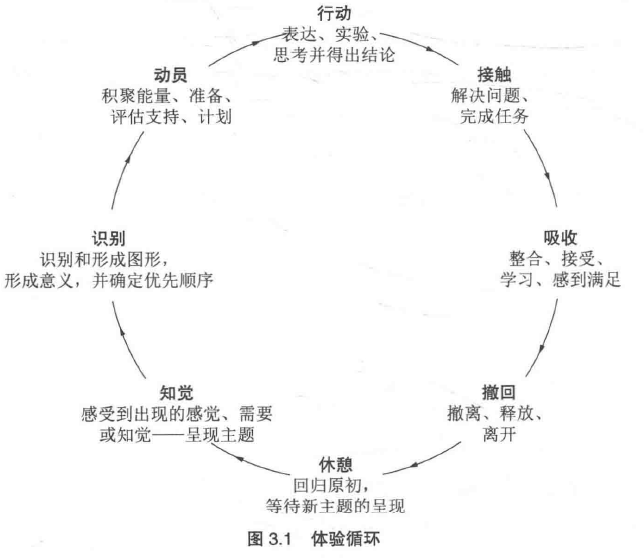
\includegraphics[width=\textwidth-11em]{aimg/2022-0406-1.jpg}
    \vspace{3pt}
\end{minipage}

\blockquote{
……一个居心叵测的女商人,刚刚完成一个收益颇丰的项目,立即就马不停蹄地寻找下一个项目或机会,无法享受闲暇,总担心如果顺其自然就会不进则退。(撤回与等待新图形出现之间的阻断)。

……一个循环完成之后到下一个主题呈现之前的阶段。这个阶段有时被称为“充实的休憩”( fertile void)。如此命名是为了强调纯粹的“存在于斯(being there)”,对自我保持充分而持续的觉察蓄势待发。……这是一种无欲、无知的状态,是主动放弃生物基本的控制欲望,也是完全放弃对未知的思维、情感、欲望、甚至信念的防御。

\citebook{格式塔咨询与治疗技术(第三版)}
}

沉默就像是休憩状态\pozhehao{}回归原初,等待新主题的呈现。在另一本书《弗里茨·皮尔斯:格式塔之父》里,fertile void被翻译为“盈空”\pozhehao{}“字面意思是‘丰富的空’,中译引用《道德经》中‘大盈若冲,其用不竭’的‘盈’字来表意‘fertile’。”

我会想起,在冥想的时候,自己也会经历一部分的体验循环,比如说知觉到一个想法或情感的出现,识别到那个想法或情感具体是什么,但没有动员、行动、接触和吸收,而是主动地撤回\pozhehao{}将自己的意识拉回到原来的锚点上(可以是自己的呼吸、周围的鸟鸣声等),然后进入盈空的状态:一片什么想法、什么情感都没有的虚无,甚至连自我意识的存在都消失了\pozhehao{}无我的状态。然后脑海里又会出现新的想法或情感,再继续这一体验循环。

但我想,冥想对于很多人而言并不是一种寻常的经历,沉默也是。

不过我也会想到,为什么是“盈空”,而不是“空”。

\blockquote{
尽管没有觉察到任何特别的东西,但这个人处于警觉状态,对所有的可能性开放。他的兴趣可能去向任何方向,此处亦或他方。他在平衡中,处于中间。他就任其自然。场还没有分化,图形和背景还是一体。

……在东方宗教中“无”(nothingness)意味着没有什么是实在的:只有过程、发生、纯粹的存在。现象学和存在主义哲学家也探索过“无”的概念,无来源于一种存在性恐惧,这种恐惧是因为意识到每个个体都是孤独的,终极意义并不存在而产生的。很多西方的普通人害怕并避免无的体验。存在主义思想认为,否认焦虑、死亡和无的现实的人,生活得不真实,皮尔斯受到这种思想的影响,提出面对存在性空可能是找到个人真实的手段。

皮尔斯不回避空,而是鼓励人们进入它并了解它。在他的第一本书中他用了一整章来教读者倾听其内在的寂静\pozhehao{}一种类似冥想的练习。他相信内在的寂静可以帮助一个人与其存在的更深的、直觉的层面接触。二十多年后,皮尔斯仍然用诗化的语言谈论空:“我们发现当我们接受、进人这种无、这个空的时候,沙漠开始开花。虚幻的空开始活跃,被充满。荒芜的空开始变成盈空。”

\citebook{格式塔咨询与治疗技术(第三版)}
}

“盈”可能更像是在指可能性的丰盈,虚无里蕴含着任何可能性的出现。只有经历了空,才会有新的体验循环,否则只是在循环着旧的体验,例如忙于开启看似新的话题、忙于和看似和新的恋人开始一段爱情,忙于追求一些看似不同却本质相同的体验。在同一个主题的体验循环里不断循环,体验变得僵硬,僵化为特定的、固定的模式。
